%-------------------------------------------------------------------------------
% LATEX TEMPLATE PRESENTATIE
%-------------------------------------------------------------------------------
% Dit template is voor gebruik door studenten van de de bacheloropleiding 
% Informatica van de Universiteit van Amsterdam.
% Voor informatie over presenteren, zie 
%                               https://practicumav.nl/presenteren/index.html
%
%-------------------------------------------------------------------------------
%	PACKAGES EN CONFIGURATIE
%-------------------------------------------------------------------------------
% Gebruik de optie "sidebar" voor toevoeging van een sidebar met inhoudsopgave
% en de optie "dyslexic" voor gebruik van het OpenDyslexic-lettertype
\documentclass[aspectratio=169,sidebar]{uva-inf-presentation}
\usepackage[english]{babel}
\usepackage{listings}
\usepackage{hyperref}
\usepackage[usenames,dvipsnames]{xcolor}

% Vul hieronder de gevraagde gegevens in, 
% meerdere auteurs en UvAnetID's gescheiden door een puntkomma 

% ouderwetseIn de video ouderwetste manier vs video
% resultaten grafiek duidelijker maken en misschien niet de andere zoekmethoden doen


% N enzo bij resultaten erbij zetten
% DER en moeilijke dingen enzo in laatste slide na conclusie kort uitleggen/ defineren

\title{AI-Driven Retrieval and Analysis of Videotaped Council Meeting Archives using Automatic Speech Recognition, Speaker Identification, and Retrieval Augmented Generation} 
\authors{Pepijn van WIjk}
\uvanetids{13952072}
\course{Bachelor thesis}
\tutor{}
\docent{Dr. Maarten Marx} 
\group{}
\programme{Informatica}

\begin{document}
%-------------------------------------------------------------------------------
%	AUTOMATISCHE SLIDES
%-------------------------------------------------------------------------------
\begin{titelframe}
\titlepage
\end{titelframe}

\title{AI-Driven Retrieval and Analysis of \colorbox{yellow}{Videotaped Council Meeting Archives} using Automatic Speech Recognition, Speaker Identification, and Retrieval Augmented Generation} 
\begin{titelframe}
\titlepage
\end{titelframe}

\title{\colorbox{yellow}{AI-Driven Retrieval} and Analysis of Videotaped Council Meeting Archives using Automatic Speech Recognition, Speaker Identification, \colorbox{yellow}{and Retrieval Augmented} \colorbox{yellow}{Generation}}
\begin{titelframe}
\titlepage
\end{titelframe}

\title{AI-Driven Retrieval and \colorbox{yellow}{Analysis} of Videotaped Council Meeting Archives using \colorbox{yellow}{Automatic Speech Recognition, Speaker} \colorbox{yellow}{Identification}, and Retrieval Augmented  Generation}
\begin{titelframe}
\titlepage
\end{titelframe}


\title{AI-Driven Retrieval and Analysis of Videotaped Council Meeting Archives using Automatic Speech Recognition, Speaker Identification, and Retrieval Augmented Generation} 
% \begin{titelframe}\frametitle{Contents}
% \tableofcontents
% \end{titelframe}

%-------------------------------------------------------------------------------
%	PRESENTATIE SLIDES
%------------------------------------------------------------------------------

% \section{Problem}
% \begin{frame}{Problem}
%     \begin{itemize}
%         \item Wet Open Overheid
%         \item Tweede Kamer publishes reports
%         \item Difficult for hundreds of local governments
%         \item journalist writing about a local meeting decision
%     \end{itemize}
% \end{frame}


\begin{frame}{Searching through meetings}
    \begin{quote}
        What are the expected advantages to the installation of the gardens surrounding underground trash containers?
    \end{quote}
\end{frame}

% Een vraag van de test doen, de verschillen in zoektochten laten zien ezno
\section{Demo}
\begin{frame}\frametitle{Demo}
\href{http://localhost:5173/\#/gemeente/ridderkerk/vergaderingen/2022/986115}{localhost}

\href{https://videotulen.wooverheid.nl/\#/gemeente/ridderkerk/vergaderingen/2022/986115}{online}
\end{frame}

\section{How we solved the problem}
\begin{frame}{How we solved the problem}
    \begin{itemize}
        \item Automatic archiving tool
        \item Automatic analysis of meetings
        \begin{itemize}
            \item Speech to text
            \item Speaker segmentation
        \end{itemize}
        \item Transcript search engine
        \item Conversation-style chat bot
        \item Easy navigable web application
    \end{itemize}
\end{frame}

\section{Methodology}
\begin{frame}\frametitle{Architecture}
\begin{figure}
    \centering
    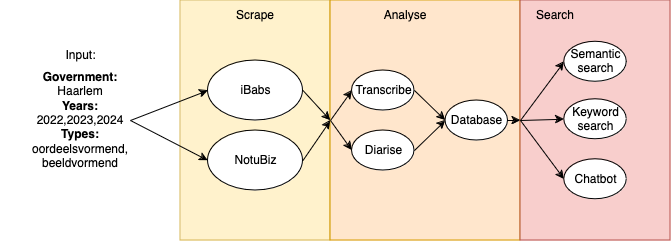
\includegraphics[width=0.99\textwidth]{images/arch.png}
    \caption{Schematic architecture of the developed analysis- and search system}
    \label{fig:pipeline}
\end{figure}
\end{frame}

% \begin{frame}\frametitle{Scraper}
% \begin{itemize}
%     \item iBabs \& NotuBiz
%     \item Downloads videos
%     \item Downloads agendas when available
%     \item Organizes archive based on year and meeting type
% \end{itemize}
% \end{frame}

% \begin{frame}\frametitle{Architecture}
% \begin{figure}
%     \centering
%     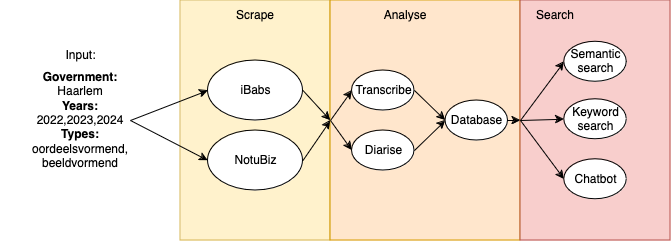
\includegraphics[width=0.99\textwidth]{images/arch.png}
%     \label{fig:pipeline}
% \end{figure}
% \end{frame}

\begin{frame}\frametitle{Analysis}
\begin{itemize}
    \item Speech to text
    \begin{itemize}
        \item OpenAI's Whisper
    \end{itemize}
    \item Speaker recognition
    \begin{itemize}
        \item pyannote.audio
    \end{itemize}
    \item Manual speaker naming
    \item Database
\end{itemize}
\end{frame}

\begin{frame}\frametitle{Analysis pipeline}
\begin{figure}
    \centering
    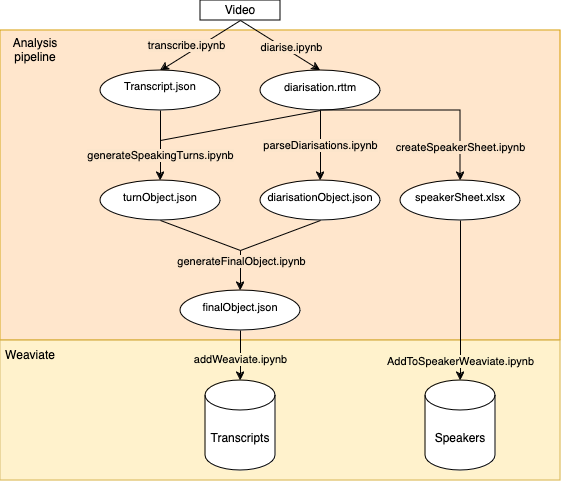
\includegraphics[width=0.53\textwidth]{images/pipeline.png}
    \caption{Schematic architecture of the developed analysis pipeline}
    \label{fig:pipeline}
\end{figure}
\end{frame}

\begin{frame}\frametitle{Architecture}
\begin{figure}
    \centering
    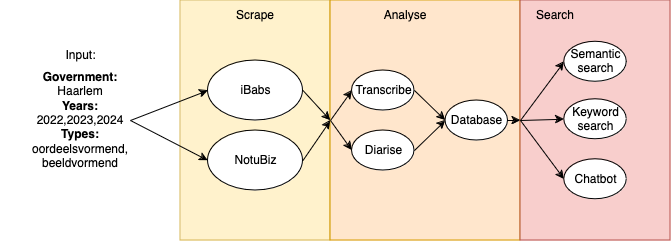
\includegraphics[width=0.99\textwidth]{images/arch.png}
    \caption{Schematic architecture of the developed analysis- and search system}
    \label{fig:pipeline}
\end{figure}
\end{frame}

% \section{Results}
% \begin{frame}\frametitle{Transcription results}
% \begin{figure}
%     \centering
%     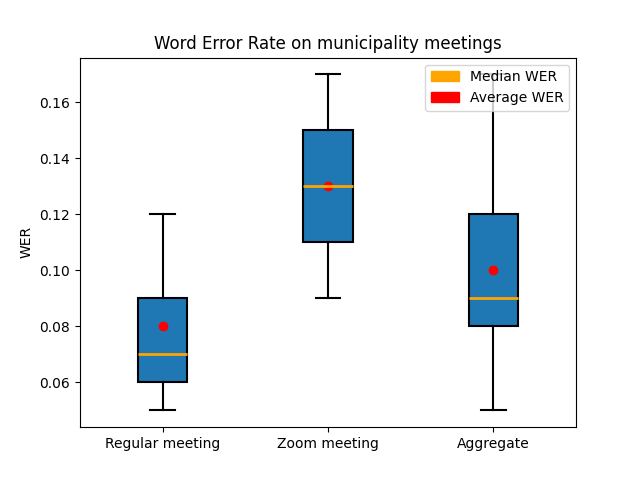
\includegraphics[width=0.67\textwidth]{images/whisperBench.png}
%     \label{fig:pipeline}
% \end{figure}
% \end{frame}

% \begin{frame}\frametitle{Diarisation results}
% \begin{figure}
%     \centering
%     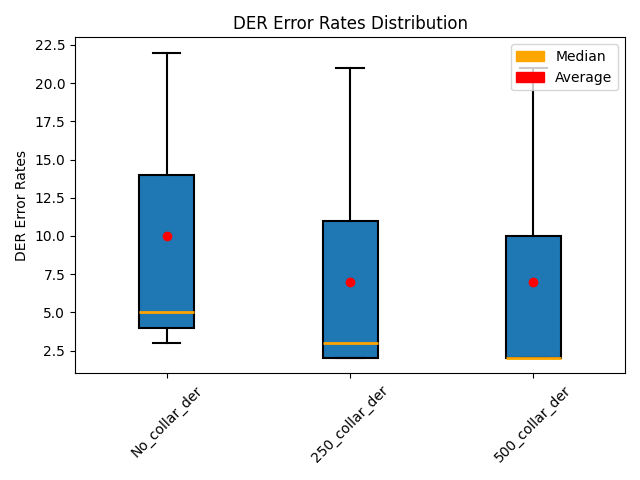
\includegraphics[width=0.65\textwidth]{images/der_error_rates_box_plot.png}
%     \label{fig:pipeline}
% \end{figure}
% \end{frame}

\begin{frame}\frametitle{Does our solution work?}
\begin{figure}
    \centering
    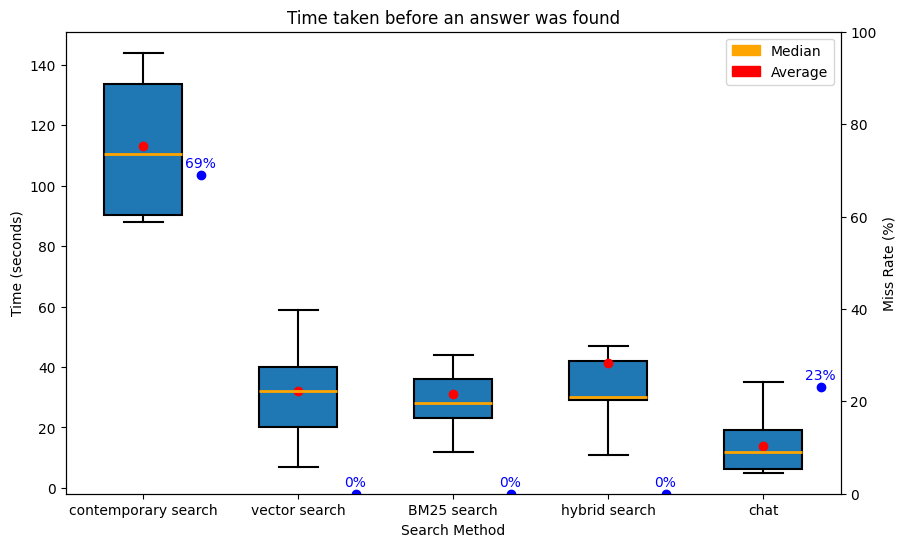
\includegraphics[width=0.6\textwidth]{images/search_engine_results_2.png}
    \caption{Average search time for different search methods used by 13 participants. Participants were given three minutes to find the answer to one of five questions.}
    \label{fig:pipeline}
\end{figure}
\end{frame}


\section{Conclusion}
\begin{frame}\frametitle{Conclusion}
\begin{itemize}
    \item Hard to navigate and find information through multi-hour long municipal meetings
    \begin{itemize}
        \item Automatic iBabs \& NotuBiz scrape tools
        \item Speaker diarisation \& automatic speech recognition
        \item Semantic- and keyword search engine
        \item Chat bot
        \item Online search application
    \end{itemize}
\end{itemize}
\end{frame}

%-------------------------------------------------------------------------------
\end{document}
